
\documentclass[11pt, reqno]{article}   	% use "amsart" instead of "article" for AMSLaTeX format
\usepackage{my_packages}

\title{PCRTBP Invariant Manifolds}
\author{Shankar Kulumani}
\date{3 July 2017}							% Activate to display a given date or no date

\begin{document}
\maketitle
%\subsection{Periodic Orbits and Invariant Manifolds}
%Used to generate a Periodic orbit about a lagrange point
%Periodic orbits about the lagrange points
%\subsection{\Poincare Section}
%Intersection of states with a lower dimensional plane
%Introduce invariant manifolds
\subsubsection{Invariant Manifolds and \Poincare Map} 
% discuss usefulness and basic generation of invariant manifolds

%Planar problem has four dimensional phase space
%associated with periodic solutions about lagrange equilibrium points
%tubes, invariant manifolds are four dimenionsal surface which serve to separate classes of trajectories
%Localized linear analysis, Monodromy matrix, is used to study and compute invariant manifold

% intro to invariant manifolds
Dynamics systems theory has been applied to design control-free maneuvers in the restricted three-body problem~\cite{koon2011}.
As previously introduced in~\Cref{sec:jacobi}, there exist five equilibrium points in the equations of motion for the three-body problem.
It has been shown that the local orbit structure near the Lagrange points gives rise to families of periodic orbits as well as the stable and unstable manifolds of these periodic orbits.
This rich structure is globally connected and gives rise to a dynamical chain which allows trajectories to pass through the phase space~\cite{koon2011,conley1968}.
The manifold structure associated with periodic orbits about the \( L_1 \) and \( L_2 \) Lagrange points are critical to the understanding of the motion of spacecraft as well as comets/asteroids.
In addition, the stable and unstable manifolds serve as the boundaries of the phase space region that allow for the transport between realms in a single three-body system or between multiple three-body systems.
These invariant manifolds only exist as a result of the dynamic formulation of the three-body problem in a rotating reference frame. 

\subsection{Invariant Manifolds}\label{sec:invariant_manifold}
% technical definition of manifold and some equations
Invariant manifolds serve as a higher dimensional generalization of the concept of seperatrices from linear systems as applied to the case of nonlinear systems. 
To compute these manifolds first one must determine an appropriate periodic orbit. 
The process of differential correction and numerical continuation are used to determine a periodic orbit with a desired energy level. 
Let the trajectories of the equations of motion defined in~\cref{eqn:cont_dyn} be defined by the flow map \( \phi(t;\vecbf{x}_0) \) originating from \( \vecbf{x}(t_0) = \vecbf{x}_0 \) and we define a periodic orbit as \( \gamma\).
The invariant manifolds are defined as : 
\begin{align*}
        W^s ( \vecbf{x}_0 ) &= \braces{ \vecbf{x} : \phi(t;\vecbf{x}_0) \to \gamma \text{ as } t \to \infty} , \\
        W^u ( \vecbf{x}_0 ) &= \braces{ \vecbf{x} : \phi(t;\vecbf{x}_0) \to \gamma \text{ as } t \to -\infty} .
\end{align*}
The stable manifold, \( W^s(\vecbf{x}_0) \), is the set of trajectories which asymptotically approach the periodic orbit.
Similarly, the unstable manifold, \( W^u(\vecbf{x}_0) \), is the set of trajectories which asymptotically depart the periodic orbit.
For the nonlinear system, defined by~\cref{eqn:cont_dyn} or~\cref{eq:discrete_eoms}, we can determine the state transition matrix \( \Phi \) along the periodic orbit, from \( 0 \to T\), by numerical integration of the variational equations.
In the neighborhood of the periodic orbit \( \gamma \), the tangent spaces to the stable and unstable manifolds are provided by the generalized eigenspaces \( E^s \) and \( E^u \) of the linearization \( A = \D f(\vecbf{x}_0) \), where \( \vecbf{x}_0 \) is on the periodic orbit.
The eigenvectors of the monodromy matrix, \( M = \Phi(T) \), serve to locally approximate the directions of the stable and unstable manifolds. 
A perturbation in the direction of the unstable eigenvector, with \( \norm{\lambda} > 1 \), is used to generate an initial condition on the unstable manifold. 
Similarly, a perturbation in the direction of the stable eigenvector, with \( \norm{\lambda} < 1 \), is used to generate an initial condition on the stable manifold. 
Each periodic orbit has two stable and unstable manifold sets associated with both a positive or negative perturbation along the respective eigenvector.
This technique of determining the invariant manifolds is graphically presented in~\cref{fig:invariant_manifold}.
\begin{figure}
        \centering
        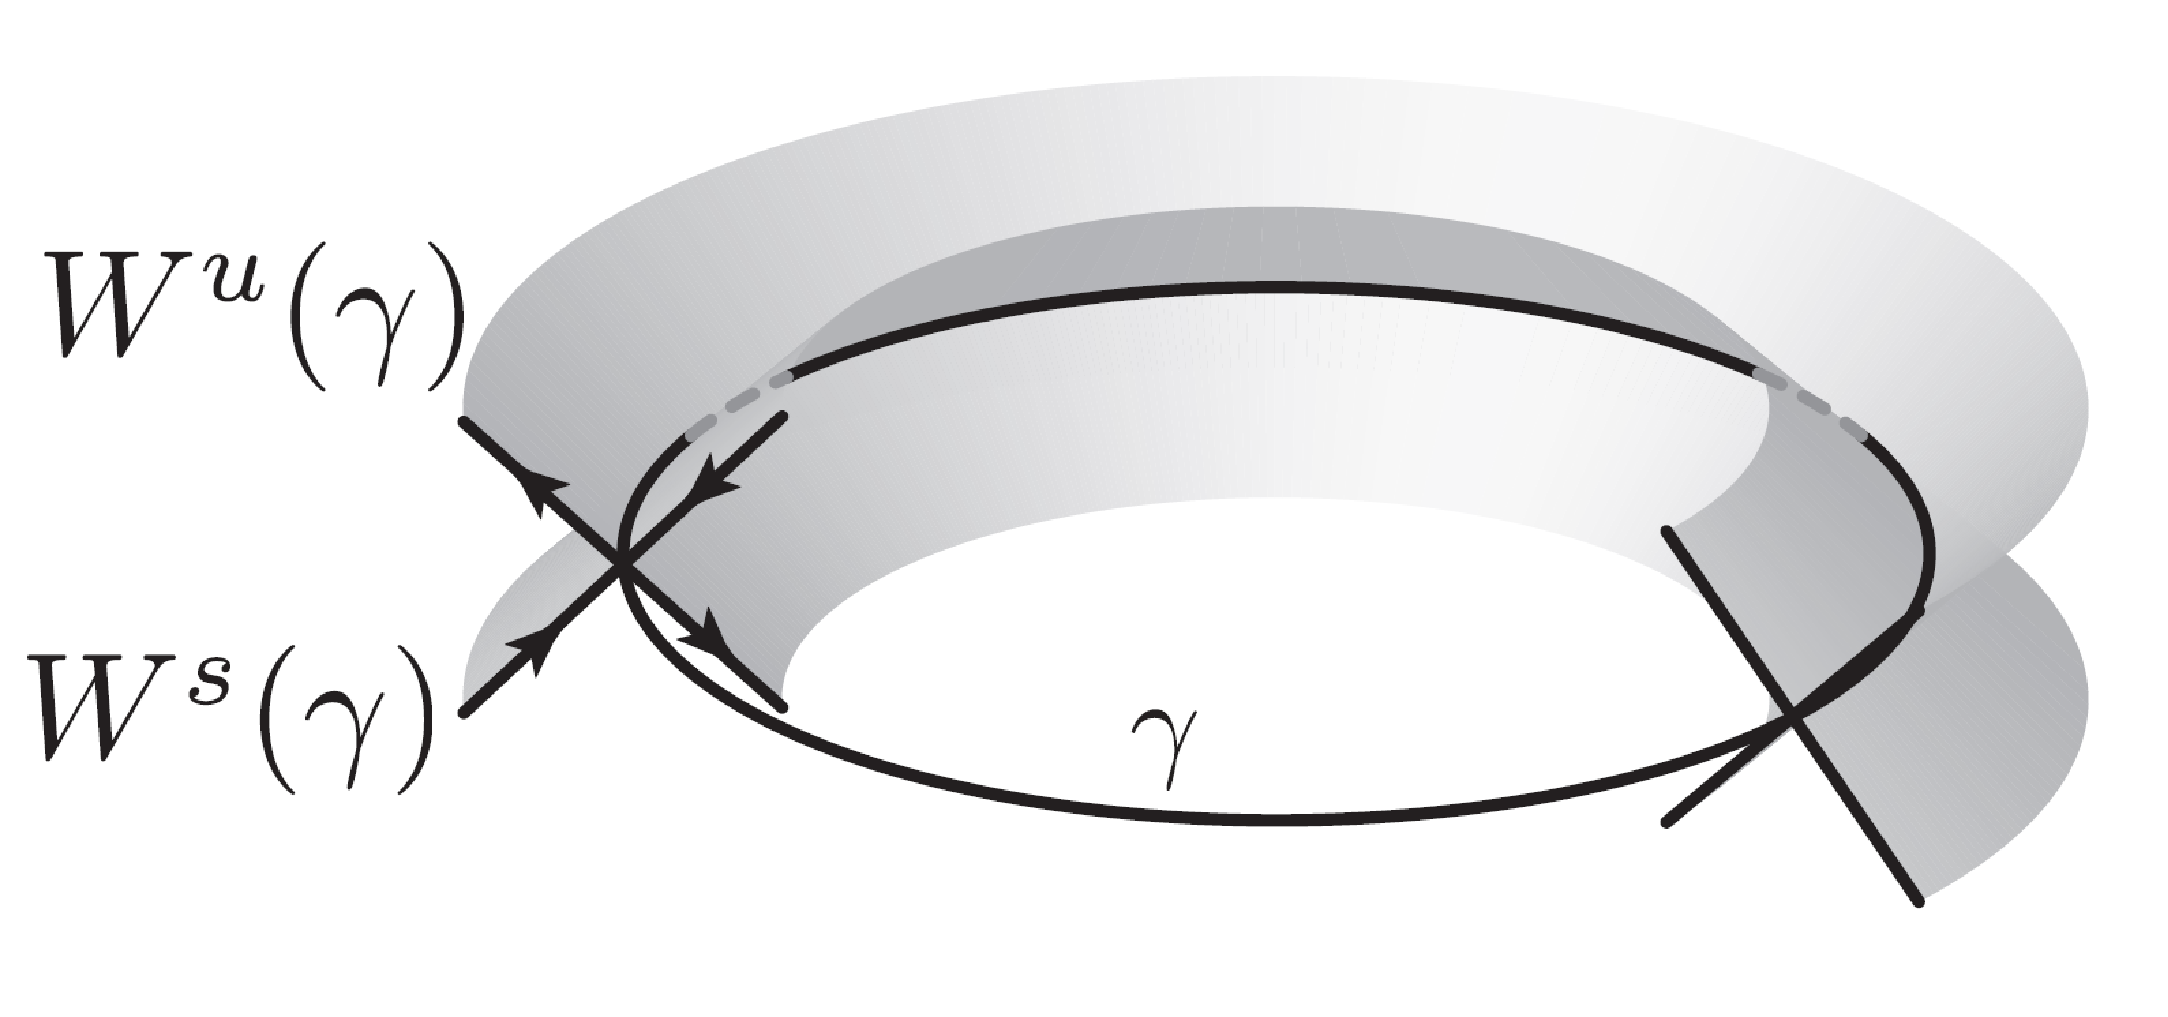
\includegraphics[width=0.5\textwidth]{invariant_manifold}
        \caption{Stable and unstable manifold of a periodic orbit\label{fig:invariant_manifold}}
\end{figure}

% introduce \Poincare section theory and math
\Poincare maps are a useful tool in the analysis of the flow near periodic orbits in the three-body problem.
We let \( \Sigma \) define a hypersurface of section chosen such that all trajectories in the vicinity of a state \( \vecbf{q} \in \Sigma \) cross \( \Sigma \) transversely and in the same direction.
A \Poincare map, \( P(\vecbf{q}) = \phi(T;\vecbf{q}) \), maps the state of a trajectory from one intersection to the next.
Choosing a section in this manner results in a \Poincare section as shown in~\cref{fig:poincare_map}.
This allows for greater insight into the stability and dynamics of periodic solutions of a dynamic system as a fixed point on the \Poincare section corresponds to a periodic orbit while movement on the section is associate with the stability of neighboring trajectories. 
For example, \Poincare maps have been used to prove the existence of homoclinic orbits, which are orbits both forward and backward asymptotic to a single unstable periodic orbit, and heteroclinic orbits, which join different periodic orbits~\cite{conley1968,koon2000b}.
These dynamic features have been shown to play a vital role in the movement of natural bodies as well as critical for spacecraft missions~\cite{gomez2001,lo1997}.
\begin{figure}
        \centering
        \begin{scaletikzpicturetowidth}{0.5\textwidth}
    \begin{tikzpicture}[tdplot_main_coords,
      poincare/.style={opacity=.2,very thick,fill=blue},
      orbit/.style={very thick,black},
      orbit hidden/.style={very thick,dashed},
      grid/.style={very thin,gray!50},
      axis/.style={->,blue,thick}, scale=\tikzscale]

    % nodes for the poincare section
    \node[label=above:\(\Sigma\)] (upper_right) at (0,5,5) {};
    \node[] (upper_left) at (0,1,5) {};
    \node[] (lower_left) at (0,1,0) {};
    \node[] (lower_right) at (0,5,0) {};

    % draw poincare section
    \draw[poincare] (upper_right.center) -- (upper_left.center) -- (lower_left.center) -- (lower_right.center) -- (upper_right.center);
    
    % draw a periodic orbit
    \coordinate (center) at (0,0,2);
    \node[below right] (x0) at (0,2,2) {\(\vecbf{q}_0\)};
    \filldraw (0,2,2) circle (3pt);

    \node[below right] (x1) at (0,3,2) {\(\vecbf{q}_1\)};
    \filldraw (0,3,2) circle (3pt);

    \tdplotdrawarc[orbit hidden]{(center)}{2}{90}{190}{}{};
    \tdplotdrawarc[orbit,<-]{(center)}{2}{-170}{90}{}{};

    \tdplotdrawarc[orbit hidden]{(center)}{3}{90}{199}{}{};
    \tdplotdrawarc[orbit,<-]{(center)}{3}{-161}{90}{}{};

        \end{tikzpicture}
    \end{scaletikzpicturetowidth}
        \caption{Diagram of the \Poincare map\label{fig:poincare_map}}
\end{figure}

\subsection{Control-free Orbital Transfers}\label{sec:control-free_transfers}
% intersect invariant manifolds on poincare section
% find intersection between stable and unstable manifolds
% define the sections used in Koon2011 (placed strategically near heteroclinic points) - rotation of manifolds
Combining invariant manifolds and an appropriate \Poincare section provides a conceptually simple manner to determine trajectories which connect wide regions of the phase space.
\Cref{fig:manifold_transfer_example} demonstrates how a \Poincare map may be used to determine a connection between periodic orbits.
The initial orbit is a planar periodic orbit about \( L_2 \) in the Earth-Moon system while the final orbit is a periodic orbit about \( L_1 \).
Both periodic orbits have the same Jacobi energy constant and as a result it is possible to transfer between the orbits without any energy change.
\Cref{fig:manifolds} shows the unstable manifold of the initial orbit and the stable manifold of the desired orbit. 
Both invariant manifolds are globalized and propogated to the first intersection with the \Poincare surface of section located at the position of the Moon, \( x = 1 - \mu \).
The \Poincare section in~\cref{fig:manifold_transfer_example} is defined as
\begin{align*}
        \Sigma = \braces{ ( y, \dot{y}) \, | \, x = 1- \mu, y > 0} , 
\end{align*}
and located to allow an intersection between both invariant manifolds.
The configuration space of the invariant manifold is \( \vecbf{x} \in \R^4 \).
The surface of section, and the resulting intersection of the four-dimensional space with the hyperplane \( \Sigma \), reduces the resulting intersection to a surface in \( \R^3\).
Since the two orbits share the same Jacobi constant, the intersection phase space is further reduced to \( \R^2\).
The intersection of the invariant manifolds on the \Poincare section is central to determining transfer connections between the initial and final orbits.

% describe this specific poincare section and why it's placed and the axes
The position, \( y \), and velocity, \( \dot{y} \), at the \Poincare section are plotted in~\cref{fig:poincare}.
The surface of section is placed at a strategic location in order to allow for a cross section of the flow within the three-dimensional energy surface. 
In a frame aligned with the rotating frame, \( ( \hat{e}_1, \hat{e}_2 ) \), but centered on the equilibrium point \( L_1 \) or \( L_2\), the unstable manifolds are locally moving in forward time in the second and forth quadrant. 
Similarly, the stable manifold branches are locally moving in backward time in the first and third quadrants as illustrated in~\cref{fig:invariant_manifold}. 
As a result, the location of the section in~\cref{fig:poincare} is chosen to intersect both the stable manifolds of \( L_1 \) periodic orbits as well as unstable manifolds of \( L_2 \) periodic orbits.
Additional \Poincare sections are located at other heteroclinic points in the phase space to enable design throughout the phase space~\cite{koon2011}.
In this way, it is possible to design trajectories that intersect the invariant manifolds and connect widely separated regions of the state space. 
This technique has been heavily investigated in~\cite{koon2011}, applied to operational missions in~\cite{koon1999}, and applied to potential multi-moon orbiter missions in~\cite{tanaka2011}.
In addition, much recent work has focused on potential return missions to the Moon~\cite{zanzottera2012,campagnola2012,mingotti2011,ozimek2010a,mingotti2009}.
\begin{figure}
     \centering
        \begin{subfigure}[b]{0.5\textwidth}
                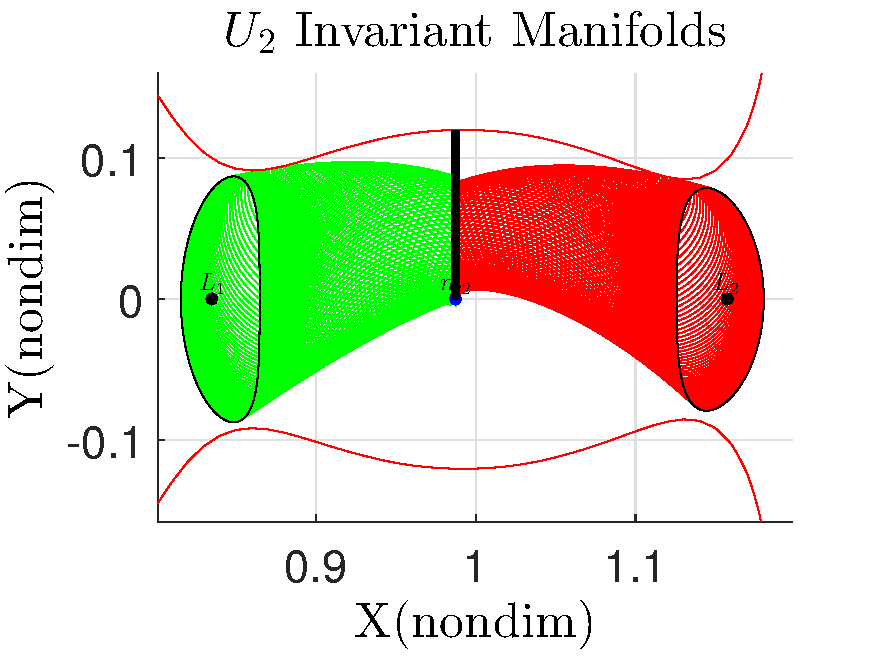
\includegraphics[width=\columnwidth]{U2_Manifolds}
                \caption{Invariant manifolds }
                \label{fig:manifolds}
        \end{subfigure}%
        ~
        \begin{subfigure}[b]{0.5\textwidth}
                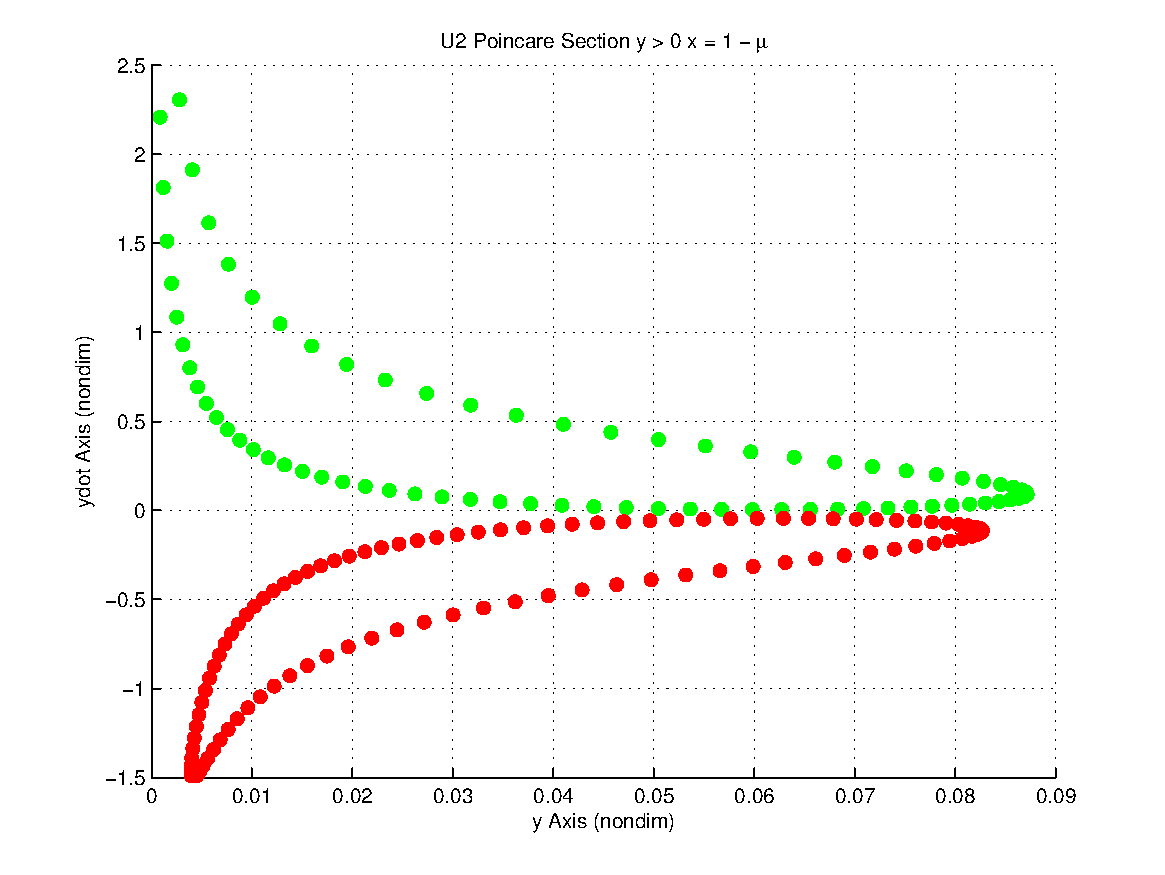
\includegraphics[width=\columnwidth]{U2_poincare}
                \caption{\(U_2\) \Poincare section}
                \label{fig:poincare}
        \end{subfigure}
        \caption{Illustration of process to identify transfer trajectories}
        \label{fig:manifold_transfer_example}
\end{figure}

% drawbacks of this approach on how we seek to improve upon it
However, the results previously developed are highly case specific and difficult to generalize to arbitrary transfers.
Also, these results are based on control-free trajectories which rely on the underlying structure of the three-body system.
In addition, transfer orbits along an invariant manifold require large time of flights which may be undesirable for time critical missions.
The addition of low-thrust propulsion offers the potential of reduced transit times and the ability to depart from the free motion trajectory to allow for increased transfer opportunities. 
In this paper, we formulate an optimal control problem to generate the reachable set of the spacecraft.
We compute the reachable set on an appropriate \Poincare section and use this to design a transfer trajectory.

\bibliographystyle{abbrv}
%\bibliography{../../../../docs/technical_papers/bibtex/library}
\bibliography{library}
\end{document}  
